%!TEX root = ../template.tex
%Developed using Sublime Text 3 with LaTexTools plugin
%SUPER+b for compiling latex to pdf
%Don't forget to use SUPER+R to jump between top level commands!
%F6 to spell check
%%%%%%%%%%%%%%%%%%%%%%%%%%%%%%%%%%%%%%%%%%%%%%%%%%%%%%%%%%%%%%%%%%%%
%% chapter4.tex
%% UNL thesis document file
%%
%% Chapter with the info about the available data
%%%%%%%%%%%%%%%%%%%%%%%%%%%%%%%%%%%%%%%%%%%%%%%%%%%%%%%%%%%%%%%%%%%%
\chapter{Proposed Approach}
\label{cha:available_data}
% ================
% = Introduction =
% ================

For this dissertation's work, it's proposed a CRISP-DM methodology to approach the problem. An explanation about this methodology is presented in section \ref{sec:crispdm}, following a suggested working plan for this dissertation in section \ref{sec:work_plan}. In section \ref{sec:available_data} the available data is presented and its quality is discussed, referring that an additional dataset is expected.

As off the time this document is being written, the Business Understanding phase has already finished and the current focus is on the Data Understanding and the Data Preparation.

\todo[inline]{na parte de utilização das tecnicas, ser mencionado de forma suave o que é cada técnica}



\section{Cross Industry Standard Process for Data Mining} % (fold)
\label{sec:crispdm}

\Acrfull{crispdm} is an iterative data mining process model that describes commonly used approaches that data mining experts use to tackle problems, which was developed by analysts representing Daimler-Chrysler, SPSS, and NCR. \Acrshort{crispdm} provides a nonproprietary and freely available standard process for fitting data mining into the general problem-solving strategy of a business or research unit.

In this methodology, a data mining project has a life-cycle consisting in six phases, where the next phase in the sequence often depends on the outcomes associated with the previous phase - making it an adaptive methodology, where the sequence of the phases is not strict and moving back and forth between different phases is always required.

The iterative nature of \Acrshort{crispdm} provides a continuous approach for cases when the solution to a particular business or research problem leads to further questions of interest, which may then be attacked using the same general process as before.


\begin{figure}[htbp]
	\centering
	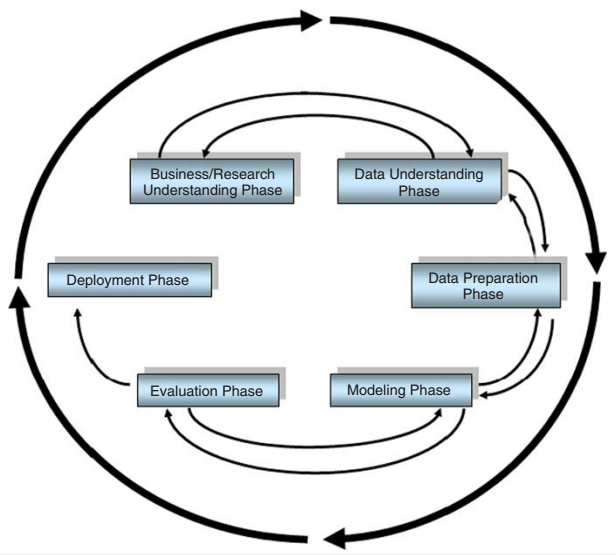
\includegraphics[width=4.5in ]{crispdm}
	\caption{\Acrshort{crispdm} process}
	\label{fig:crispdm}
\end{figure}

\subsection{CRISP-DM phases}
\label{subsec:crispdm_phases}

\subsubsection{Business/Research Understanding}
\label{subsubsec:business_understanding}

This initial phase focuses on clearly enunciate the project objectives and requirements in terms of the business or research unit as a whole. Then, it is necessary to convert this knowledge into a data mining problem definition, so that a preliminary strategy is made for achieving these objectives.

\subsubsection{Data Understanding}

This phase starts with the collection of the data to proceed with activities in order to get familiar with the data. The next step is evaluate the quality of the data and get the firsts insights. Finally, if desired, interesting subsets can be selected that may contain actionable patterns to form hypotheses for hidden information.

\subsubsection{Data Preparation}

This labor-intensive phase covers all aspects of preparing the final data set, which shall be used for subsequent phases, from the initial raw data. Data preparation tasks are prone to be performed multiple times, and not in any prescribed order. Tasks include selecting cases and variables to analyse, perform transformations on certain variables, and clean the raw data so that it is ready for the modeling tools.

\subsubsection{Modeling}

In this phase, the goal is to select and apply appropriate modeling techniques for further parameters' calibration to optimal value. Typically, several techniques may be applied for the same data mining problem. Some techniques have specific requirements on the form of data. Therefore, looping back to data preparation phase is often required.

\subsubsection{Evaluation}

At this stage in the project you have built a model (or models) that were delivered from Modeling phase. These models must be evaluated for quality and effectiveness, before they can be deploy for use in the field.
Before the deployment, it is also necessary to determine whether the model in fact achieves the objectives set for it in phase \ref{subsubsec:business_understanding}. Another key objective in this phase is to establish whether some important business issue has not been sufficiently accounted for. At the end of this phase, a decision on the use of the data mining results should be reached.

\subsubsection{Deployment}

Although this is the last phase, the creation of the model is generally not the end of the project. Depending on the requirements, the deploy can be as simple as generating a report or as complex as implementing a repeatable data scoring or data mining process. For businesses, the customer often carries out the deployment based on the analyst model.


\section{Work Plan} % (fold)
\label{sec:work_plan}

According to the CRISP-DM methodology, the first phase of this dissertation consisted on the study of three phase circuits and \acrshort{ims}, as well as understanding the several problems that affect them and the associated state of the art. The output of this phase consists on a document where the basics of three phase circuits can be learned from the perspective of a Computer Scientist, plus the problem definition which this dissertation is approaching. The next steps consist on data preparation and modeling, where an iterative approach will be done by interweaving the study of Signal Processing (\ref{subsec:data_prep_studying_signal}) and Machine Learning techniques (\ref{subsec:modeling_under_machine_learning}). 
After the experience and knowledge acquired through phase \ref{subsec:data_prep_studying_signal} and \ref{subsec:modeling_under_machine_learning} using a specific dataset, the modeling phase is expected to be re-iterated since a new dataset is expected by September. Meanwhile, an evaluation of the most promising models will be made. Although the process may be re-iterated, a prototype is expected as a result of this dissertation work.


\subsection{Understanding Induction Motors}

A focused output of this phase is summarise on chapter \ref{cha:intro_electric_motors}, where an understanding of the target motor in this dissertation can be found. A more complete output of this phase can be found on a future appendix of this document.


\subsection{Data Understanding}

At the moment, two datasets are available. One of the datasets can't be used since the sample rate of the metrics is too big to detected small fluctuations on the current to detect inter-turn short circuit between a low number of turns.
The other dataset is divided in 3 categories: healthy motor samples, faulty motor samples with 2 turns short-circuited, and faulty motor samples with 19 turns short-circuited. Its sample frequency is appropriate to detect such faults, but the sample period is merely 4 seconds long for each category and therefore doesn't have statical relevance on the lifetime of the motor. Therefore, this dataset is useful to understand the data as well as to understand the transformation that can be applied to get more insights.
It is expected that more data will be collected from several motors starting September. A more detailed section on this subject can be found on \ref{sec:available_data}.

\subsection{Data Preparation: Understanding Signal Processing}
\label{subsec:data_prep_studying_signal}

This phase will proceed in parallel with phase \ref{subsec:modeling_under_machine_learning}. Given the features available in the raw data, it is necessary to derive another set of features so that the differences between healthy stream data and faulty stream data can be found. Since the data is the representation of several signals (voltage and current), emerges the necessity to study several techniques to analysis this kind of data. For this purpose, a set of Signal Processing techniques will be study such as Fourier Analysis, several transforms (Hilbert, Wavelet, Z, Fourier), as well as several signal filters.
The transforms to study where chosen given its use in several relevant works ~\cite{M.a2014} ~\cite{Riera-Guasp2015} ~\cite{Cheng2011} and its relevance in the classical signal processing.
The goal is to experiment some features addition on the data and test some modeling techniques, while studying a specific signal processing technique and data streaming methods.

At the moment, it's still uncertain what is the best way to obtain the signal (all the points sampled over a reasonable period of time, root mean square over a reasonable period of time, what is the most reasonable sample frequency to detect the failures in near real time) and what's the best way to transform the signal (Park-Hilbert transformation, fast Fourier transformation, sparse fast Fourier transformation or wavelet transformation).


\subsection{Modeling: Understanding Machine Learning Techniques}
\label{subsec:modeling_under_machine_learning}

This phase will proceed in parallel with phase \ref{subsec:data_prep_studying_signal}. As an result of the state of the art's study, several works use Artificial Neural Networks and Support Vector Machines to detect faults ~\cite{Toma2011} ~\cite{Wolkiewicz2013} ~\cite{Patel2016} ~\cite{Jagadanand2015}. Therefore, these machine learning techniques will be study for further modeling. While developing the models, they will also be evaluated and compared with each others.  
Other techniques that will be studied are Clustering techniques.

\subsubsection{Artificial Neural Networks}
\label{subsec:ann}

\Acrfullpl{ann} are classifiers inspired by Biology. As all kind of classifiers, an \Acrshort{ann} goal is to maximize the likelihood for the predicted result of a given input to be as close as possible of the real result. This goal is accomplished by training the \Acrshort{ann} , which will adapt the consideration of the input against the expected result of that input. This classifier provides a general method for learning functions from examples, being the examples real-valued, discrete-valued, or vector-valued.

\Acrshort{ann} are composed by perceptrons, which are units that take a vector of real-valued inputs, calculates a linear combination of these inputs, and then computes a function which will give the result, as seen in figure \ref{fig:sigmoid_unit}.

\begin{figure}[htpb]
\centering
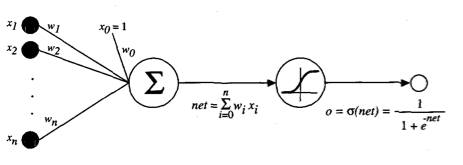
\includegraphics[width=0.5\textwidth]{sigmoidunit.png}
\caption{A perception unit with sigmoid activation function}
\label{fig:sigmoid_unit}
\end{figure}

Each perceptron have a linear combination so that a value may be produced from the input vector. from figure \ref{fig:sigmoid_unit}, it can be seen that each input has its own height. So, for example, a simple linear combination could be such as the equation \ref{eq:linear_combination}.

\begin{equation} 
\label{eq:linear_combination}
\sum_{i=1}^{n} w_{i}*x_{i}
\end{equation}

After the perceptron computes the linear combination, this value is applied to a function which will give us the class. For example, in a binary classification problem, the activation function can be the Logistic Function - also called sigmoid function.

\subsubsection{Support Vector Machine}
\label{subsec:svm}

\Acrfull{svm} is a supervised machine learning algorithm that can be used for classification and regression problems. In a binary classification context, this technique requires a labeled data set of training examples so that it can build a model that assigns new examples into one category or the other, making it a non-probabilistic binary linear classifier.
Given that training set, the \Acrshort{svm} defines the criterion to be looking for a decision surface that is maximally far away from any data point, which can be viewed in figure \ref{fig:svm_margin}. 

\begin{figure}[htpb]
\centering
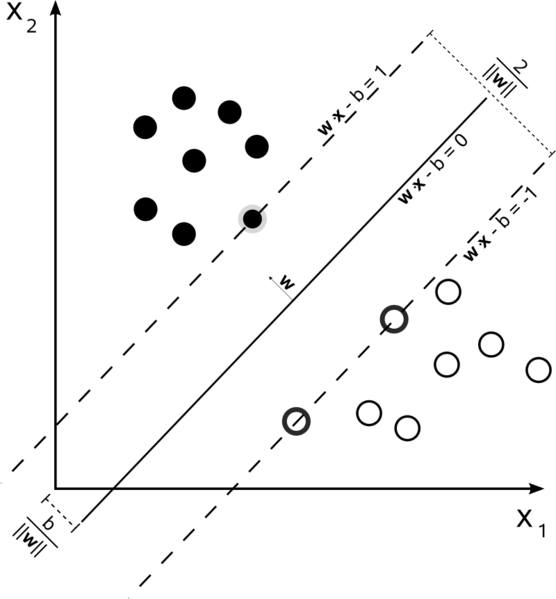
\includegraphics[width=0.5\textwidth]{Svm_max_sep_hyperplane_with_margin.png}
\caption{Margins for an SVM trained with samples from two classes}
\label{fig:svm_margin}
\end{figure}

This distance from the decision surface to the closest data point determines the margin of the classifier.

Therefore, the decision function for an \Acrshort{svm} is fully specified by a (usually small) subset of the data which defines the position of the separator, which can be seen in figure \ref{fig:svm_margin}. These points are referred to as the support vectors. They are called vectors because in a vector space, a point can be thought of as a vector between the origin and that point.

\subsection{New dataset acquisition and Modeling re-iteration}
\label{subsec:reiteration}

The new dataset will have a superset of the currently working dataset's features. Therefore, it is expected that the knowledge gained in previous phases will be valid to used and it's expected that the same input features will be used, but now the model will have a more statistical significant sample. More info about the new dataset can be found in section \ref{sec:available_data}.


\section{Available Data}
\label{sec:available_data}

As off the day of this document's writing, the available data can be divided into two categories: an unlabeled dataset containing the current, voltage and power logs of a factory's motor (data category 1) and a dataset labeled containing 3 sets of data - healthy motor, faulty motor and a more severe faulty motor (data category 2).
It is expected another set of data from several machines with turn insulation faults to arrive by September (data category 3).
The following is a summary of the two categories of data, as well as the expected data (\ref{subsec:data_category_3})

\subsection{Data Category 1}
\label{subsec:data_category_1}

This data was provided by Optisigma from one of its pilots. Each tuple in this dataset contains the timestamp, root mean square of the last 30 seconds of the voltage per phase and the  current per phase. It also contains the mean power per phase, the connection type of the motor in that time period and the mean temperature.
The provided data begins at \emph{03/02/2016  10:12:40} and ends at \emph{09/06/2016  18:05:22}.
In spite of having a good time period of data, the data is unlabeled and we cannot know if there was any kind of fault at a given time since it was not being registered by the company.
Furthermore, given the sample difference being of 30 seconds we cannot study neither the spectrum of the current neither the current over time.

From this iteration, Optisigma was informed that the available data could not be used for the purpose of this dissertation.
Therefore, it was provided another dataset (\ref{subsec:data_category_2}) so that an analysis could be made in order to understand not only the data and the conventional signal processing techniques, as well as determinate at which frequency the samples of the current and voltage should be made.

\subsection{Data Category 2}
\label{subsec:data_category_2}

This data was provided so that the conventional signal processing techniques could be study, as well as to apply other techniques that could identify the fault. This data is composed by three datasets:

\begin{itemize}
  \item 
  Dataset of a healthy motor, sampled at 18kHz during 4 seconds
  \item 
  Dataset of a faulty motor with 2 short circuited turns, sampled at 18kHz during 4 seconds
  \item 
  Dataset of a faulty motor with 19 short circuited turns, sampled at 18kHz during 4 seconds
\end{itemize}

In all the datasets, the used motor is the same.

All the datasets have the same set of features:  \textbf{time}, \textbf{current phase R}, \textbf{current phase S}, \textbf{current phase T}, \textbf{voltage RS} and \textbf{voltage ST}. A summary of the features is shown in table bla

% Please add the following required packages to your document preamble:
% \usepackage{booktabs}
\begin{table}[htpb]
\centering
\caption{My caption}
\label{my-label}
\begin{tabular}{@{}ccc@{}}
\toprule
\textbf{Feature} & \textbf{Unit} &                                                   \textbf{Data Category 2 features' description} \\ \midrule
current phase R  & Ampere        & Stator line current of phase R                    \\
current phase S  & Ampere        & Stator line current of phase S                    \\
current phase T  & Ampere        & Stator line current of phase T                    \\
voltage RS       & Volt          & Stator line-to-line voltage between phase R and S \\
voltage ST       & Volt          & Stator line-to-line voltage between phase S and T \\ \bottomrule
\end{tabular}
\end{table}


From the line-to-line voltage presented on the data, the third line-to-line voltage voltage (voltage TR) can be inferred - since it is a balanced three-phase system, the sum of the three phases has to be approximately zero. And from the line-to-line voltage, the line-to-neutral per phase voltage can be inferred.

For online signal processing, sampling with 18kHz is too high since it then brings computational complexity and such a sampling rate brings noise to the sampled signal. Therefore, a first re-sample of the data was made to reduce the sampling frequency to 1kHz. The sampling frequency will influence the max frequency that we can address on the spectrum analysis as well as the step of the analysed frequencies.

\subsection{Data Category 3}
\label{subsec:data_category_3}

It is expected of this data to have a similar schema as the data in \ref{subsec:data_category_2}, and the sample frequency will depend on the analysis of the data category refered in \ref{subsec:data_category_2}. This data is expected to be from several motors with several short circuited inter-turns, so that a more robust model could be made.